\documentclass{article}
\usepackage[utf8]{inputenc}
\usepackage{hyperref}
\usepackage{amsmath}
\usepackage{amsfonts}
\usepackage{graphicx}


\title{SPhO Ten Year Series (TYS) with Solutions: 2014 Questions}
\author{
    Solutions available on Victoris\\
    \texttt{victoris.org}
    % new collaborators add your name and contact here!
}

\date{\today}

\begin{document}
\maketitle

\section{2014}
\subsection{Question 1}
1. Yo-Yo! \\ A yo-yo of mass $M$ lies on a smooth horizontal table as shown below. The moment of inertia about the center may be taken as $\frac{1}{2} M A^{2} .$ A string is pulled with force $F$ from the inner radius $B$ as indicated below.

\begin{figure}
	\centering
	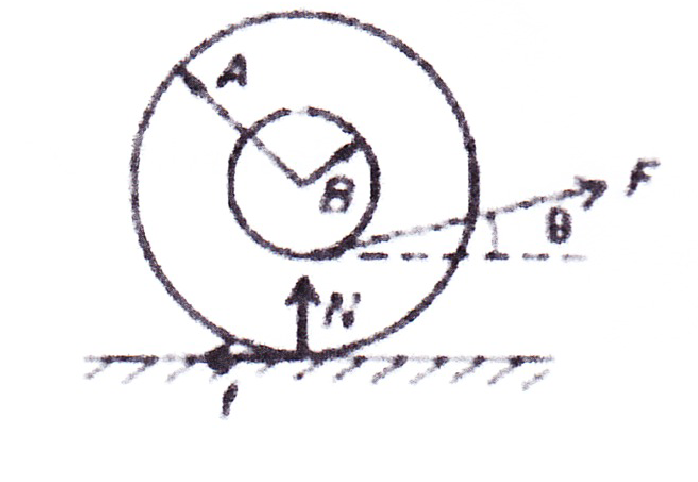
\includegraphics[width=0.5\linewidth]{spho_book_TYS_images/2014q1.png}
	\caption{Yo-yo on a smooth table}
\end{figure}

(a) Draw diagrams to show which direction the yo-yo will roll if $\theta=0, \pi / 2, \pi .$ [2] \\
(b) For what value of $\theta$ will the yo-yo slide without rolling independent of the roughness (coefficient of friction) of the table or the magnitude of $F$? [3] \\
(c) At what angle $\theta$ will the yo-yo roll, independent of the smoothness of the table? [5]

\subsection{Question 2}
2. Yo-yo continued \\ A yo-yo is pulled by its string along a horizontal surface without slipping. The horizontal velocity of the end of the string remains equal to $v .$ A bar is pivoted as shown and remains supported by the yo-yo. Find the angular speed of the bar $\omega$ as a function of the angle $\theta$. The outer and the inner radii of the yo-yo are $R$ and $r$ respectively. [10]

\begin{figure}
	\centering
	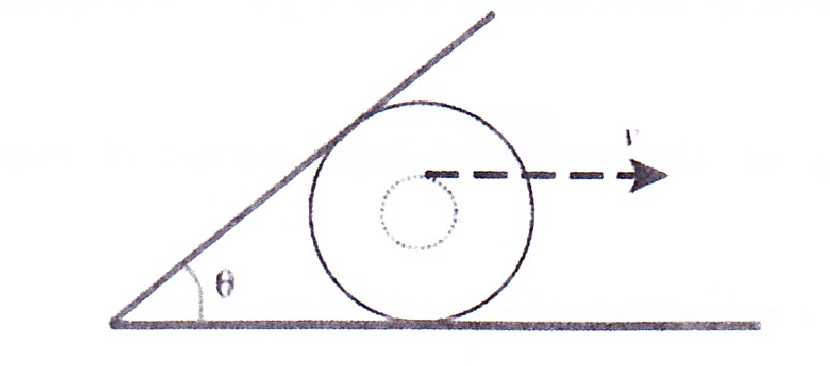
\includegraphics[width=0.5\linewidth]{spho_book_TYS_images/2014q2.png}
	\caption{Pulled yo-yo and supported bar}
\end{figure}

\subsection{Question 3}
3. Cylindrical capacitors \\
(a) A long cylindrical conductor has a radius $a$ and a linear charge density $+\lambda$. It is surrounded by a coaxial cylindrical conducting shell with inner radius $b$ and linear charge density $-\lambda .$ Calculate the capacitance per unit length for this capacitor, assuming that there is vacuum in the space between the cylinders. [4] \\
(b) Consider a cylindrical capacitor of length $l$ and of radii $a$ and $b$ as defined in (a), write down the conditions for which increasing $l$ by $10 \%$ would be more effective in increasing its capacitance than increasing $a$ by $10 \%$. [6] 

\subsection{Question 4}
4. Spring with mass \\ Problems involving springs often consider the springs to be massless. Of course, that is not true in reality. Here, we consider a spring with mass $M$, equilibrium length $L_{\circ}$, and spring constant $k$. \\
(a) The spring above has one end fixed and the other end moving with speed $v$. Assume the speed of points along the length of the spring varies linearly with distance $l$ from the fixed end. Assume also that the mass $M$ of the spring is distributed uniformly along the spring. Express the kinetic energy of the spring in terms of $M$ and $v$. [5] \\
(b) Write down the conservation of energy equation of a spring-mass system where the mass $m$ is moving at the end of a massless spring. What is the angular frequency $\omega$ for such a system? [2] \\
(c) By considering the procedure in (b), what is the angular frequency $\omega$ of the spring mentioned in (a)? If the effective mass $M^{\prime}$ of the spring is defined as $\omega=\sqrt{\frac{k}{M^{\prime}}}$ what is $M^{\prime}$ in terms of $M ?$ [3]

\subsection{Question 5}
5. Catching the wave \\
The speed of of a travelling wave $v$ along a string is a function of its tension $T$ and its linear mass density $\rho$ in the form $v=T^{\alpha} \rho^{\beta}$. \\
(a) Find $\alpha$ and $\beta$. [2] \\
(b) A uniform, almost inextensible string of length $l$ and total mass $M$ is suspended vertically and tapped at the top end so that a transverse impulse runs down it. At the same moment, a body is released from rest and falls freely from the top of the string. How far from the bottom does the body pass the impulse? [8]

\subsection{Question 6}
6. Playing with Horizontal Plates \\ A capacitor system is made of 2 horizontal square plates of sides $l$ separated by a distance $d$. \\
(a) If the uniform electric force field between them is $E$, what are the charges on the respective plates? Express your answer in terms of $E, l$ and other fundamental constansts.  [3] \\
(b) What is the force which the plates exert on each other when the potential difference between then is $V$ ? [2] \\
(c) The upper plate is fixed and the lower plate is resting on a table top and is free to move. The potential difference $V$ is gradually increased till the lower plate suddenly jumps up. Calculate the value of $V$ at which this occurs, given that the lower plate is made of alumninum (density $2.71 \times 10^{3} \mathrm{~kg} \mathrm{~m}^{-3}$ ) of thickness $8.00 \mu \mathrm{m}$ and that the initial separation is $12.7 \mathrm{~mm}$. [2] \\
(d) What is the energy per unit volume stored in the capacitor just before the lower plate jumps up? [2] 

\subsection{Question 7}
7. (a) At low temperatures, the heat capacity of a substance is dependent on its temperature. A thermally insulated piece of the substance is heated under atmospheric pressure by an electric cuurent so that it receives electric energy at a constant power $P$. This leads to an increase of the absolute temperature $T$ of the substance with time $t$ as $T(t)=T_{\circ}\left[1+a\left(t-t_{\circ}\right)\right]^{\frac{1}{3}}$. Here, $a, t_{\circ}$ and $T_{\circ}$ are constants. Determine the heat capacity $C_{p}$ of the substance as a function of temperature. [5] \\
(b) The index of refraction of glass can be increased by diffusing in impurities. It is then possible to make a lens of constant thickness. Given a disk of radius $a$ and thickness $d$, express the index of refraction $n(r)$ as a function of $n_{\circ}$ (refractive index at the centre of the lens), $r$ (radius from the centre of the lens), $d$ and $F$. You may assume $d<<a$. [5]

\subsection{Question 8}
8. (a) After falling a time $t$ in the atmosphere, an outer shell of a meteorite of thickness $x$ will have been heated significantly. The thickness can be estimated by dimensional analysis as the following thermodynamic parameters: $x=t^{\alpha} \rho^{\beta} c^{\gamma} k^{\sigma}$. \\
$\rho$ is the meteorite's density. \\
$c$ is the metorite's specific heat capacity. \\
$k$ is the meteorite's thermal conductivity. \\
Determine by dimensional analysis the value of the four powers $\alpha, \beta, \gamma$ and $\sigma$. [5] \\
(b) A beam of $10^{6} K_{l}$ mesons per second with $\beta=\frac{v}{c}=\frac{1}{\sqrt{2}}$ is observed to interact with a lead brick such that the $K_{l}$ mesons are being converted to $K_{s}$ mesons with the internal state of the lead brick identical before and after the reaction. The direction of motion of the incoming $K_{l}$ and outgoing $K_{s}$ may also be considered to be identical. Using
$$
\begin{aligned}
	&m\left(K_{l}\right)=5 \times 10^{8} \mathrm{eV} / c^{2} \\
	&m\left(K_{l}\right)-m\left(K_{s}\right)=3.5 \times 10^{-6} \mathrm{eV} / c^{2}
\end{aligned}
$$
give the magnitude and direction of the avearge force exerted on the brick by this process. [5] 

\subsection{Question 9}
9. Among the first successes of the interpretation by Ampere of magnetic phenomena, we have the computation of the magnetic field $B$ generated by wires carrying an electric current, as compared to early assumptions originally made by Biot and Savart. \\
A particularly interesting case is that of a very long thin wire, carrying a constant current $i$, made out of two rectilinear sections and bent in the form of a "V", with angular half-span $\alpha$ (see figure). According to Ampere's computations, the magnitude $\mathrm{B}$ of the magnetic field in a given point $\mathrm{P}$ lying on the axis of the "V", outside of it and at a distance $d$ from its vertex, is proportional to $\tan \left(\frac{\alpha}{2}\right) .$ Ampere's work was later embodied in Maxwell's electromagnetic theory, and is universally accepted. 

\begin{figure}
	\centering
	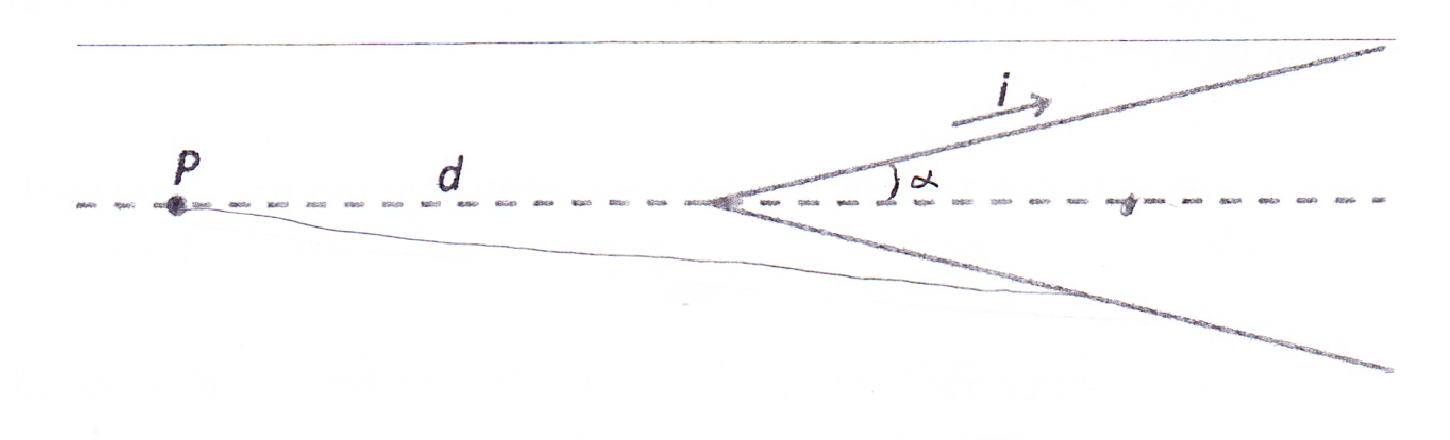
\includegraphics[width=0.5\linewidth]{spho_book_TYS_images/2014q9.png}
	\caption{Configuration of V-shaped wire}
\end{figure}

Using our knowledge of electromagnetism \\
(a) find an expression of the magnetic field $B$ in terms of the given quantities and any other relevant constants. Also, indicate the direction of the magnetic field [4] \\
(b) Compute the field at a point $\mathrm{P}^{*}$ symmetric to $\mathrm{P}$ with respect to the vertex i.e along the axis and at the same distance $d$ but inside the "V". [4] \\

\subsection{Question 10}
10. Radioactive dating of sample ${ }^{87} R b$ (element no 37) decays into the stable isotope ${ }^{87} S r$ (element no. 38) with a half life of $T_{\frac{1}{2}}=4.9 \times 10^{10}$ year, relative to the stable isotope ${ }^{86} \mathrm{Sr} .$ At the point of formation, the ratio ${ }^{87} \mathrm{Sr} /{ }^{86} \mathrm{Sr}$ was identical for all minerals in the sample while the ratio ${ }^{87} R b /{ }^{86} S r$ was quite different. As time passes on, the amount of ${ }^{87} R b$ decreases by decay, while consequently the amount of ${ }^{87} S r$ increases. As a result, the ratio of ${ }^{87} S r /{ }^{86} S r$ will be different today. In the following figure(a), the points on the horizontal line refer to the ratio ${ }^{87} R b /{ }^{86} S r$ in different minerals at the formation of the sample.

\begin{figure}
	\centering
	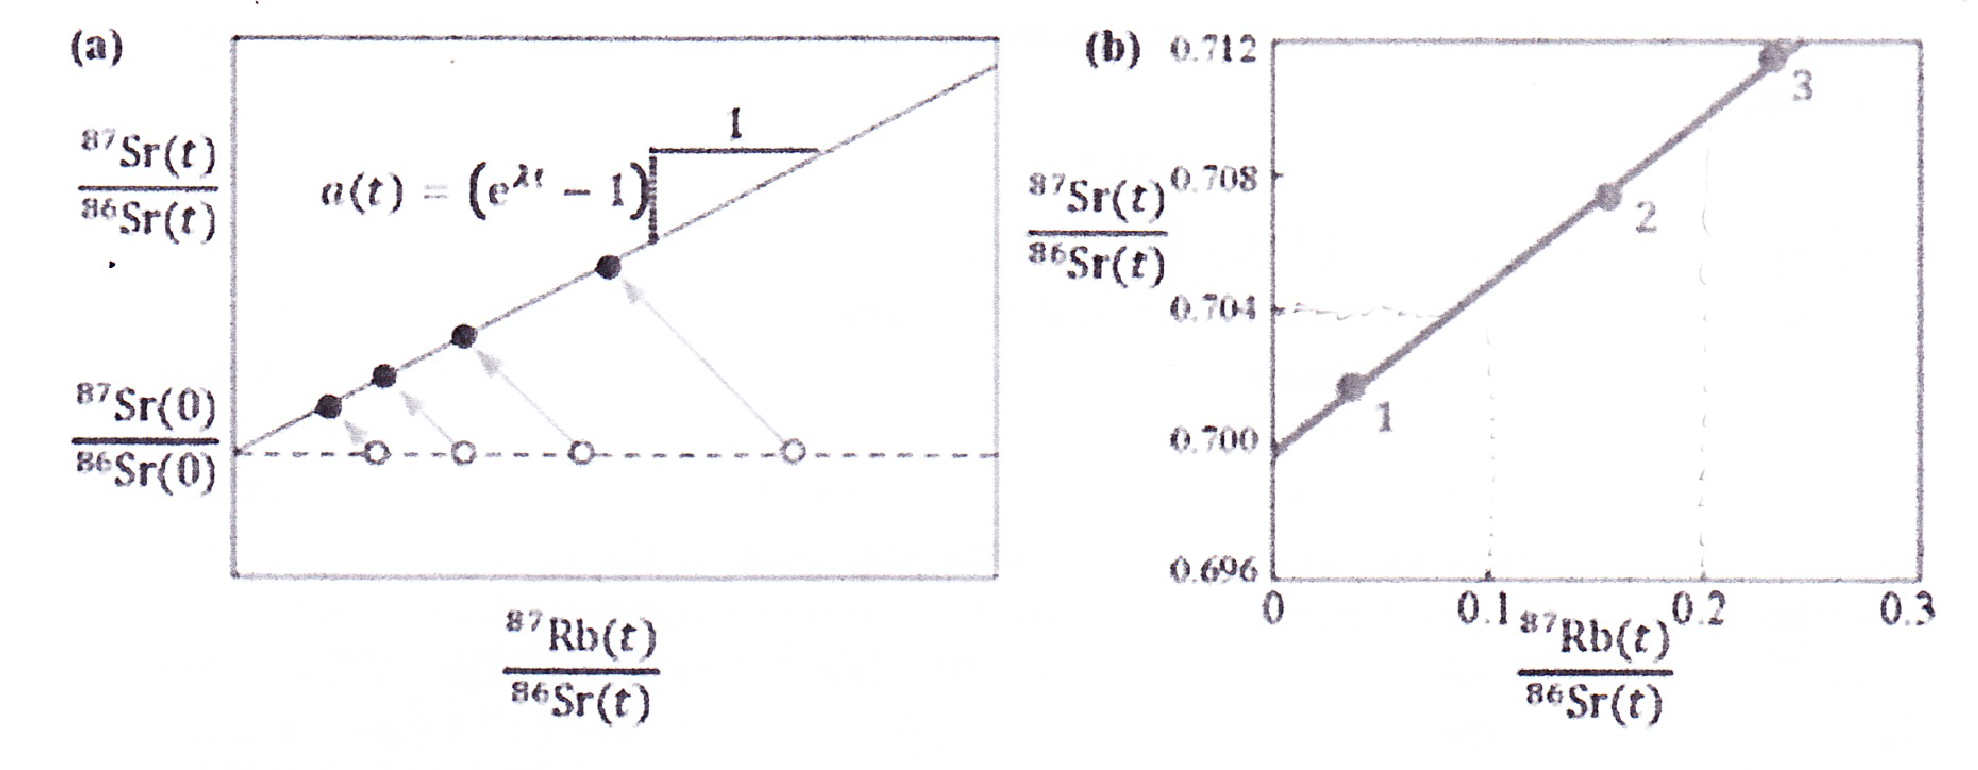
\includegraphics[width=0.5\linewidth]{spho_book_TYS_images/2014q10.png}
	\caption{(a) The ratio ${ }^{87} \mathrm{Sr} /{ }^{86} \mathrm{Sr}$ in different minerals at the time of formation, $t=0$ (open circles) and at present time (filled circles) (b) The isochron-line for three different minerals taken from the sample at present time}
\end{figure}
(a) Write down the nuclear reaction depicting the decay scheme for the transformation of ${ }_{37}^{87} R b$ to ${ }_{38}^{87} Sr$. \\
(b) Show that the present-time ratio ${ }^{87} \mathrm{Sr} /{ }^{86} \mathrm{Sr}$ was plotted versus the present-time ratio ${ }^{87} R b /{ }^{86} S r$ in different mineral samples from the same sample forms a straight line (the isochron line), with slope $a(t)=\left(e^{\lambda t}-1\right) .$ Here $t$ is the time since the formation of the minerals, while $\lambda$ is the decay constant inversely proportional to half-life $T_{\frac{1}{2}}$ \\
(c) Determine the age $\tau_{m}$ of the sample using the isochron line as in the above diagram. [3]

\end{document}
